\section{Basic selection validation with signal truth MC}
\label{app:signal-mcstudy}

Monte Carlo data on $RSG \to HH \to 4b$ is studied to validate the current methods to match Higgs to calorimeter jets and b's to trackjets. Namely, that the two leading (by \pt) calorimeter jets, each with a size of $\Delta R = 1.0$ are treated as Higgs candidates, and that the two leading trackjets (also by \pt) within each calorimeter jets are treated as the b candidates.

Large-R Jets Higgs Matching: First it is examined whether the two leading calorimeter jets match with the Higgs particles, i.e. whether each Higgs has a \DR less than 1.0 for a matching calorimeter jet. Figure \ref{fig:app-truth-Higgs} demonstrates that $\sim 95\%$ of the time, the two leading large-R jets match up with the two leading Higgs. Thus, it is not necessary to include the third leading calorimeter jet to identify the Higgs, as doing so could only improve the matching rate by $5\%$, and doing so would likely lower background rejection.

\begin{figure}[htbp!]
\begin{center}
% Old MC
%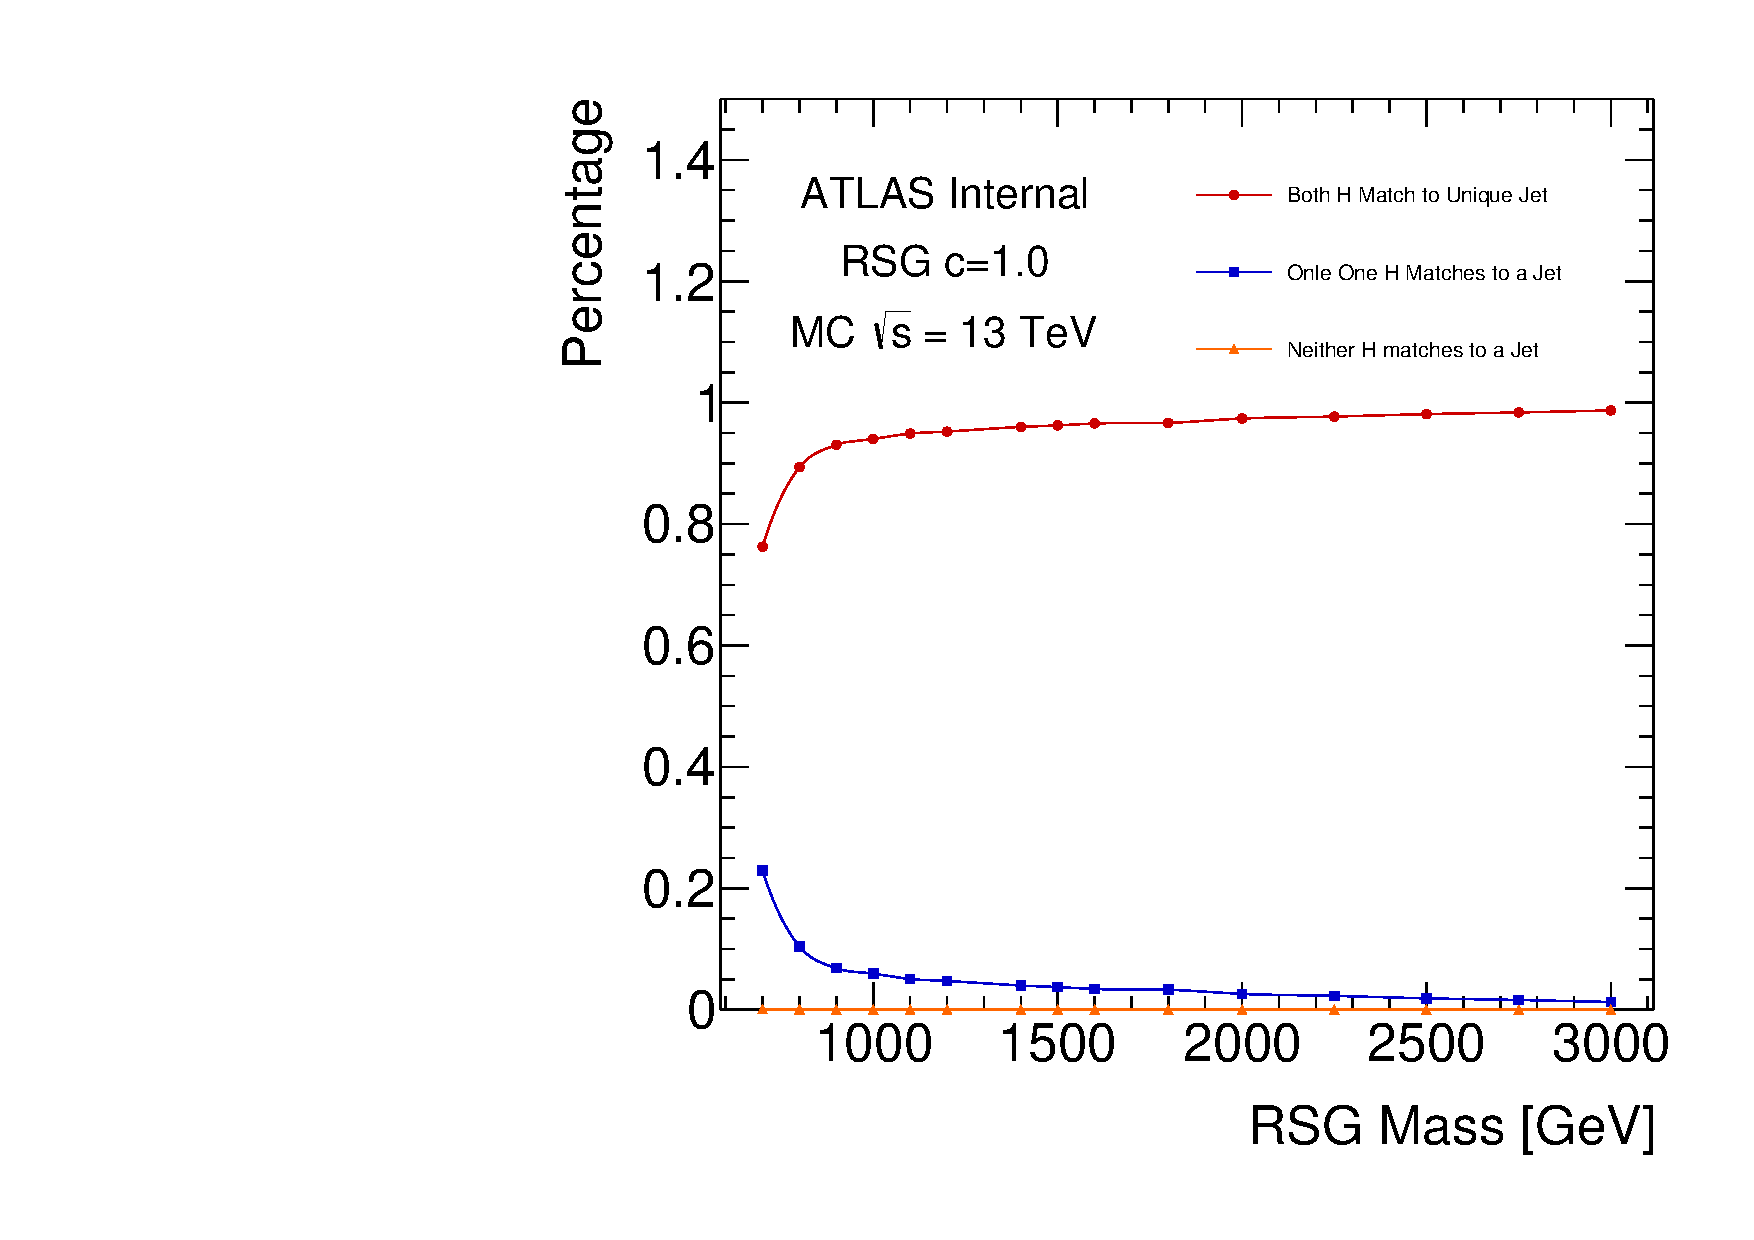
\includegraphics[scale=.48]{figures/boosted/Appendix-Truth/truth_higgs-matching.pdf}
\caption{Percentages of Higgs to Jet matching possibilities as a function of the mass of the Randall-Sundrum Graviton in Monte Carlo data. Note that the case where each Higgs gets matched to the same jet essentially never happens, so it is not included in this plot.}
\label{fig:app-truth-Higgs}
\end{center}
\end{figure}

In addition, the calorimeter jets almost always contain the $b\overline{b}$ pair that each Higgs decay into. Figure \ref{fig:app-truth-HbdR} shows that the Higgs and its leading child $b$ almost always have an angular displacement less than $1.0$, so as long as the Higgs is matched closely with a calorimeter jet, each b will also be inside that calorimeter jet. Thus, a size of $\Delta R = 1.0$, is enough to contain both b's.

\begin{figure}[htbp!]
\begin{center}
% Old MC
%\subfloat[Leading Higgs]{{%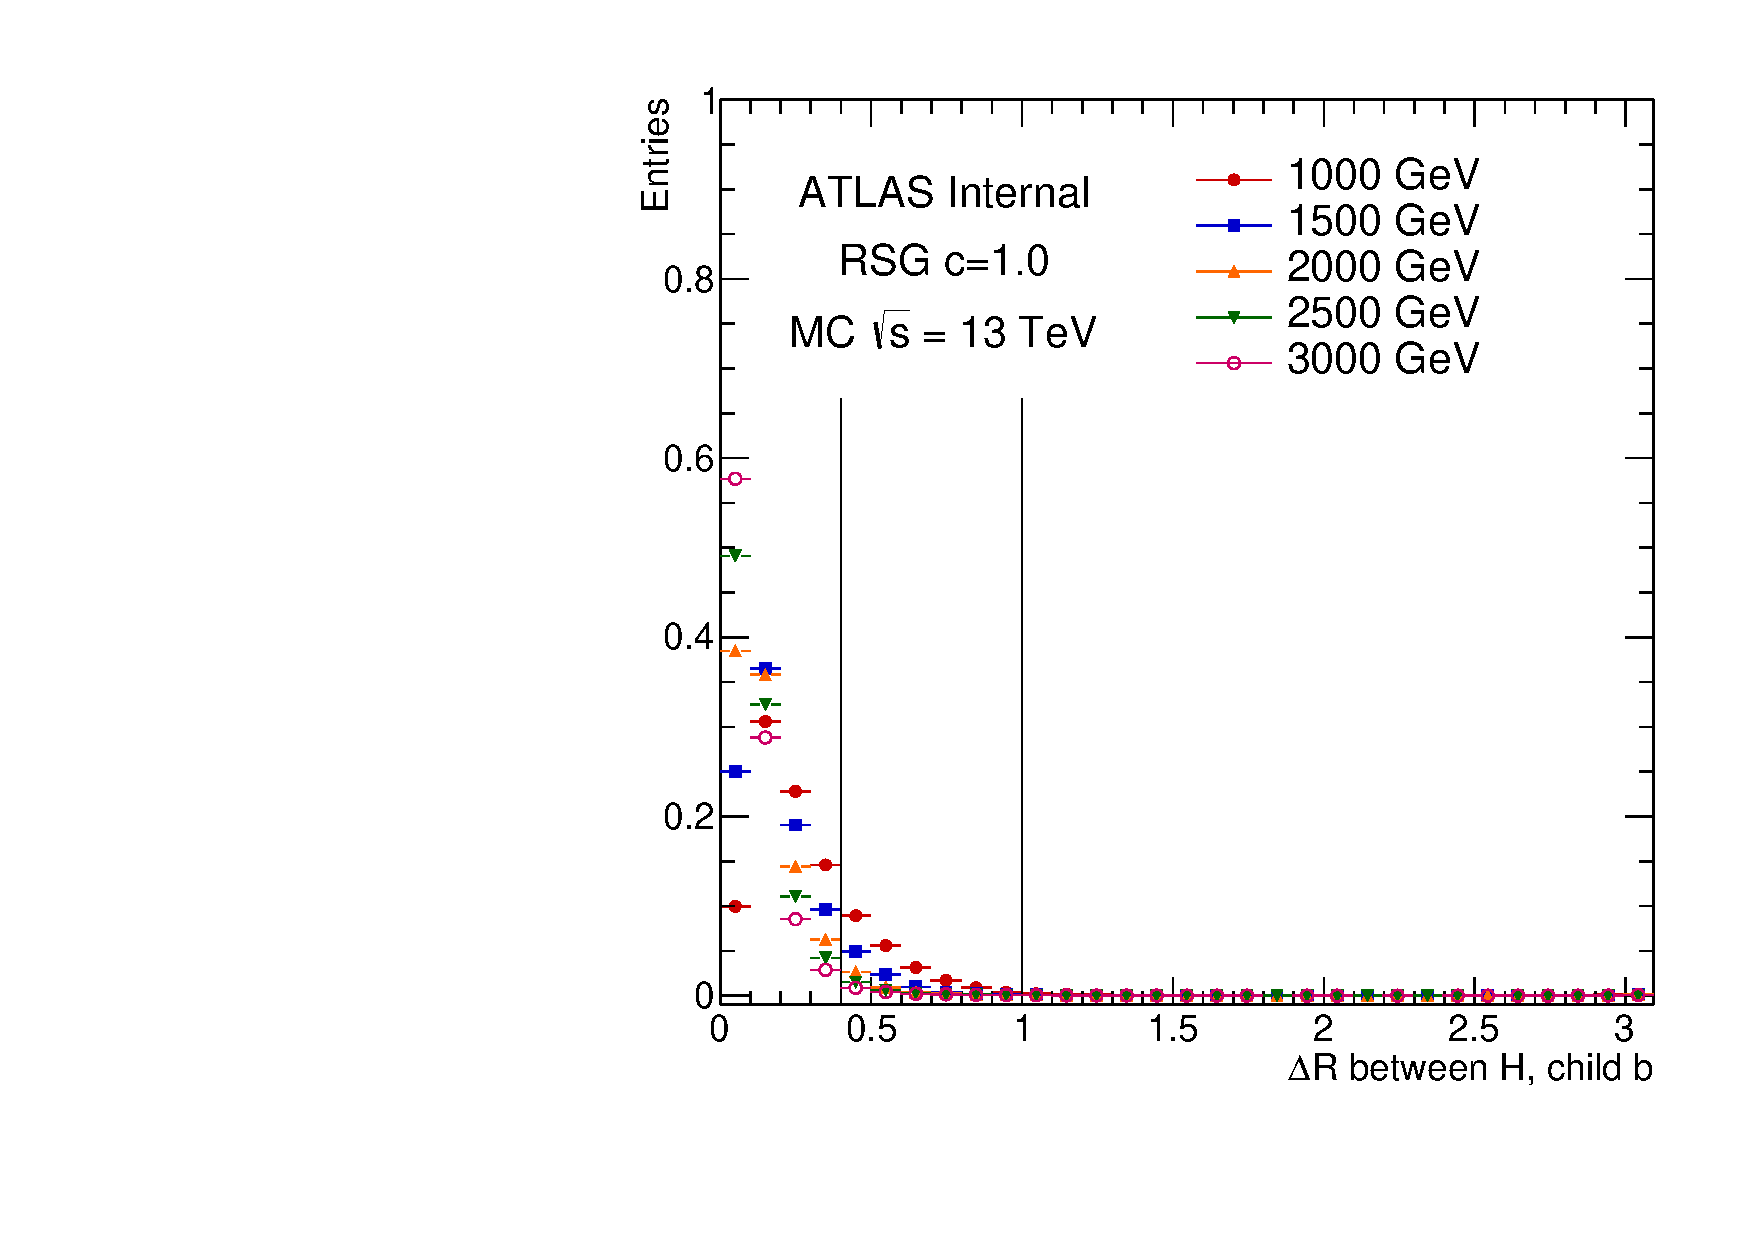
\includegraphics[angle=270, width=7cm]{figures/boosted/Appendix-Truth/truth_hbdR.pdf}}}
\qquad
%\subfloat[Subleading Higgs]{{%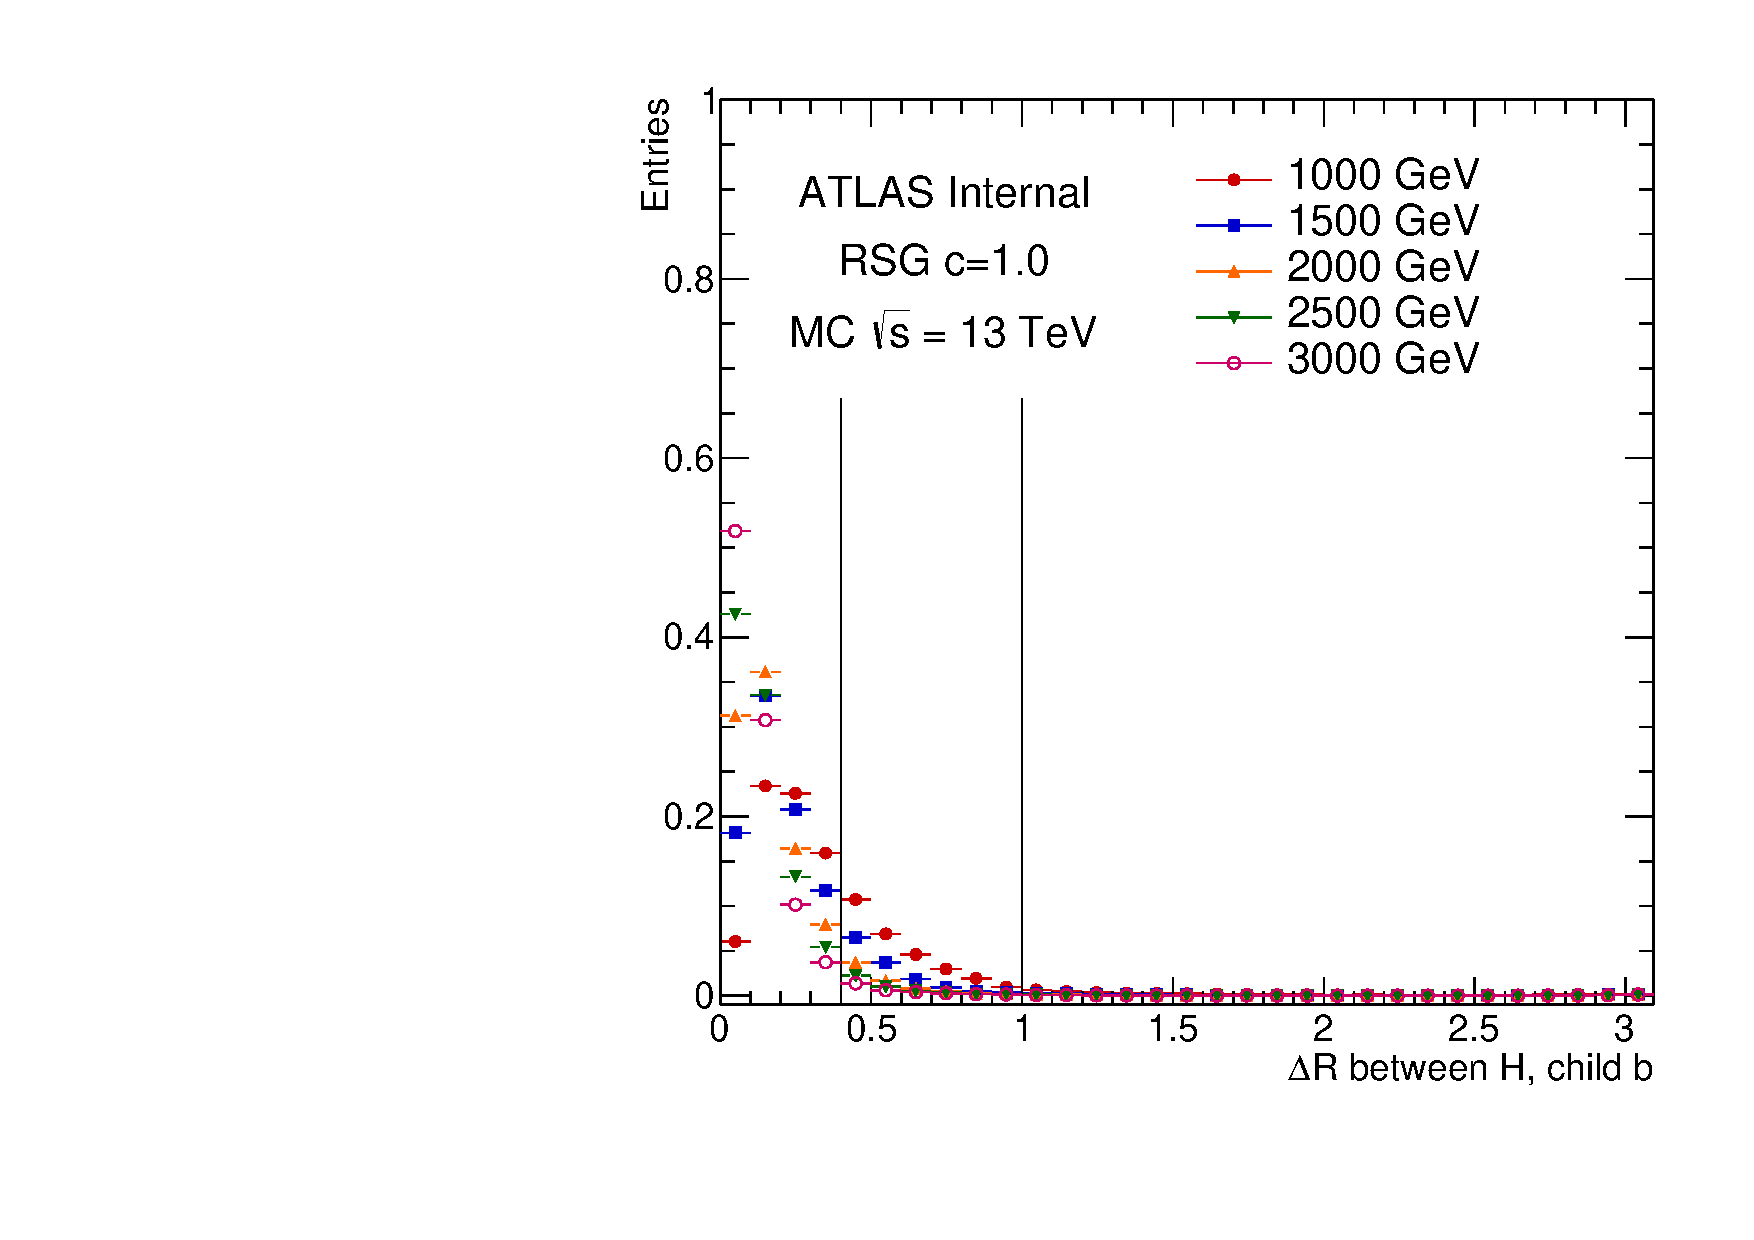
\includegraphics[angle=270, width=7cm]{figures/boosted/Appendix-Truth/truth_hbdR2.pdf} }}
\caption{$\Delta R$ between Higgs (leading by \pt on left, subleading on right) and the child b quark. Lines are drawn at $\Delta R = 0.4$ (size of large R jets for the resolved $HH \to 4b$ analysis) and $\Delta R = 1.0$ (size for boosted). }
\label{fig:app-truth-HbdR}
\end{center}
\end{figure}

Track Jets-Matching: Now that we know that the b's are contained inside the large-R jets, we can investigate whether they actually match with the track jets inside each large-R jet. Figure \ref{fig:app-truth-bmatch} shows that for low RSG mass, b's are matched to track jets about $80\%$ of the time. At high mass, the b-jets begin to merge, so at that point the b's tend to be identified with the same trackjet (this is accounted for in the Boosted analysis by the 2tag split signal region). Including a third trackjet could help only in the case where one of the b's is not matched but the Higgs is matched correctly, which happens only about $5-15\%$ of the time. Thus using the two leading trackjets is good enough for matching the b's, since including a third trackjet could improve the matching rate by at most $10\%$.

\begin{figure}[htbp!]
\begin{center}
% Old MC
%\subfloat[Leading Higgs]{{%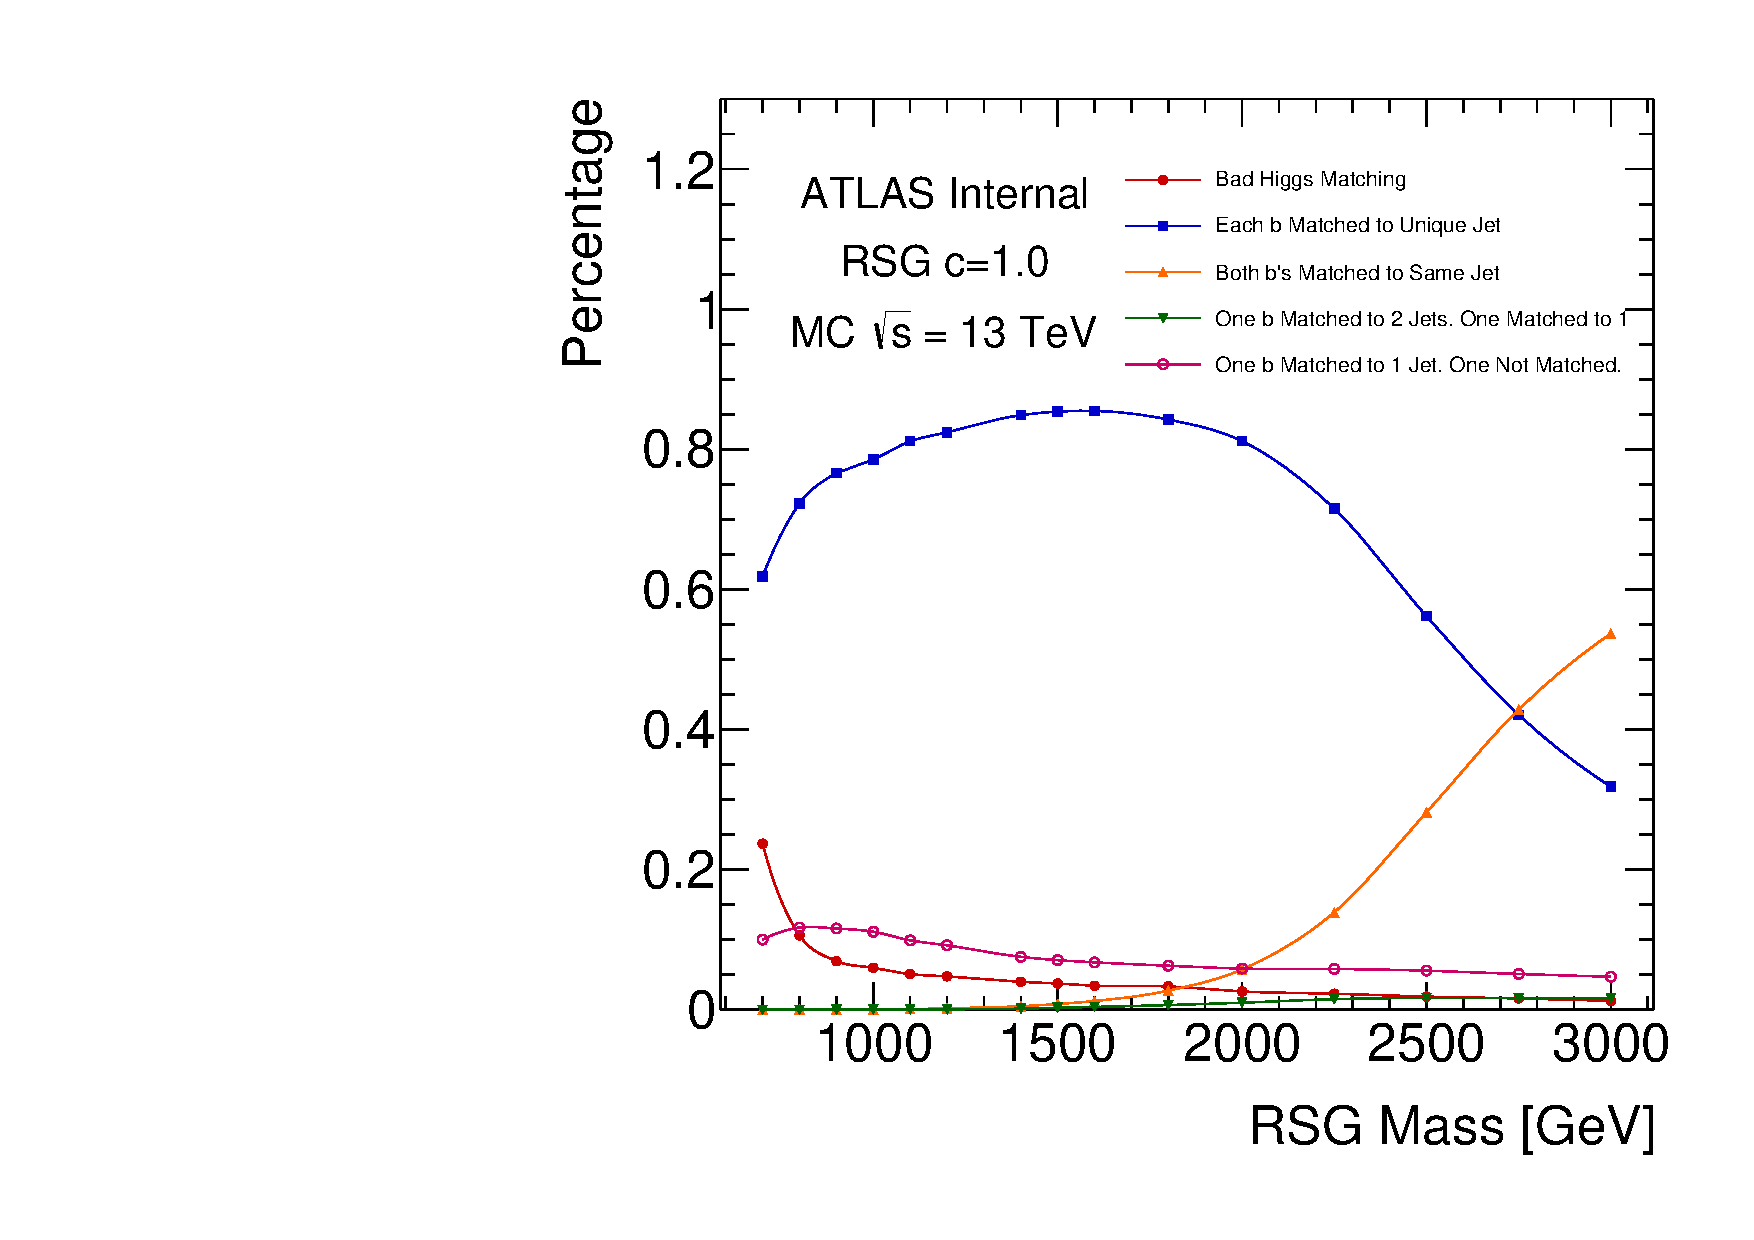
\includegraphics[angle=270, width=7cm]{figures/boosted/Appendix-Truth/truth_b-matching.pdf} }}
\qquad
%\subfloat[Subleading Higgs]{{%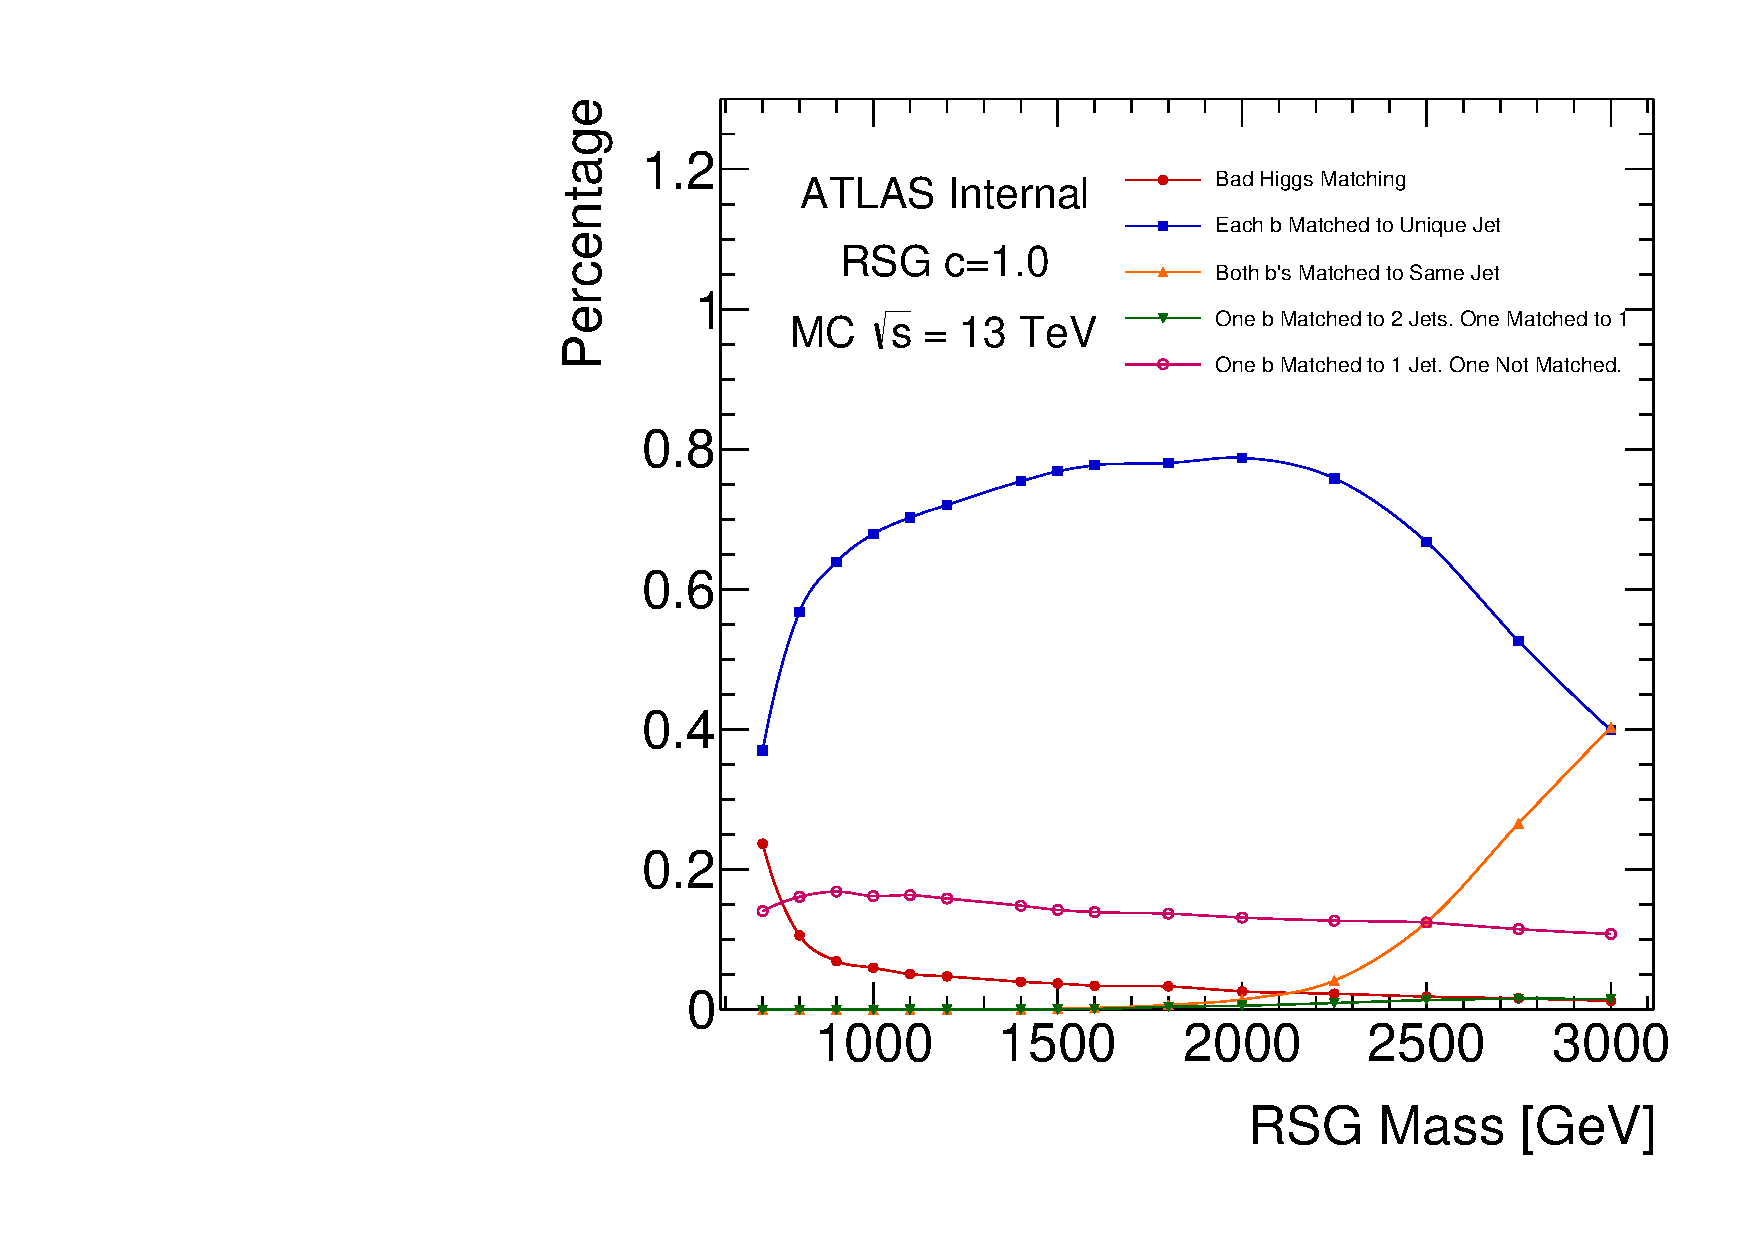
\includegraphics[angle=270, width=7cm]{figures/boosted/Appendix-Truth/truth_b-matching-sublead.pdf} }}
\caption{Percentage of the time that different combinations of matching b's to trackjets occur relative to all possible combinations of matching the $b\overline{b}$ pair to 2 trackjets (b's inside leading Higgs on left, inside subleading on right). The situations listed in the legend are all independent, but they are not comprehensive. The situations not listed on the legend (including those cases where a b is not in the calorimeter jet) happen in total at most $1.6\%$ of the time for a given mass point.}
\label{fig:app-truth-bmatch}
\end{center}
\end{figure}

b-Tagging: Finally, it is examined how often the track jets that the b's are matched to are b-tagged. B-tagging is based on (the old method) MV2c20 with a cut of $-0.6134$ (at the $77\%$ working point). B-tagging does not perform particularly well on the trackjets, especially for high RSG mass (Figure \ref{fig:app-truth-bbtag}). Note that the rise in the percentage of time that both b's are b-tagged at high RSG mass is due to the fact that the b-jets begin to merge (as shown in figure \ref{fig:app-truth-bmatch}) and because in figure \ref{fig:app-truth-bbtag} the b's are allowed to match to the same track jet. Thus, the rise is not due to an effect of the b-tagging algorithm.


\begin{figure}[htbp!]
\begin{center}
% Old MC
%\subfloat[Leading Higgs]{{%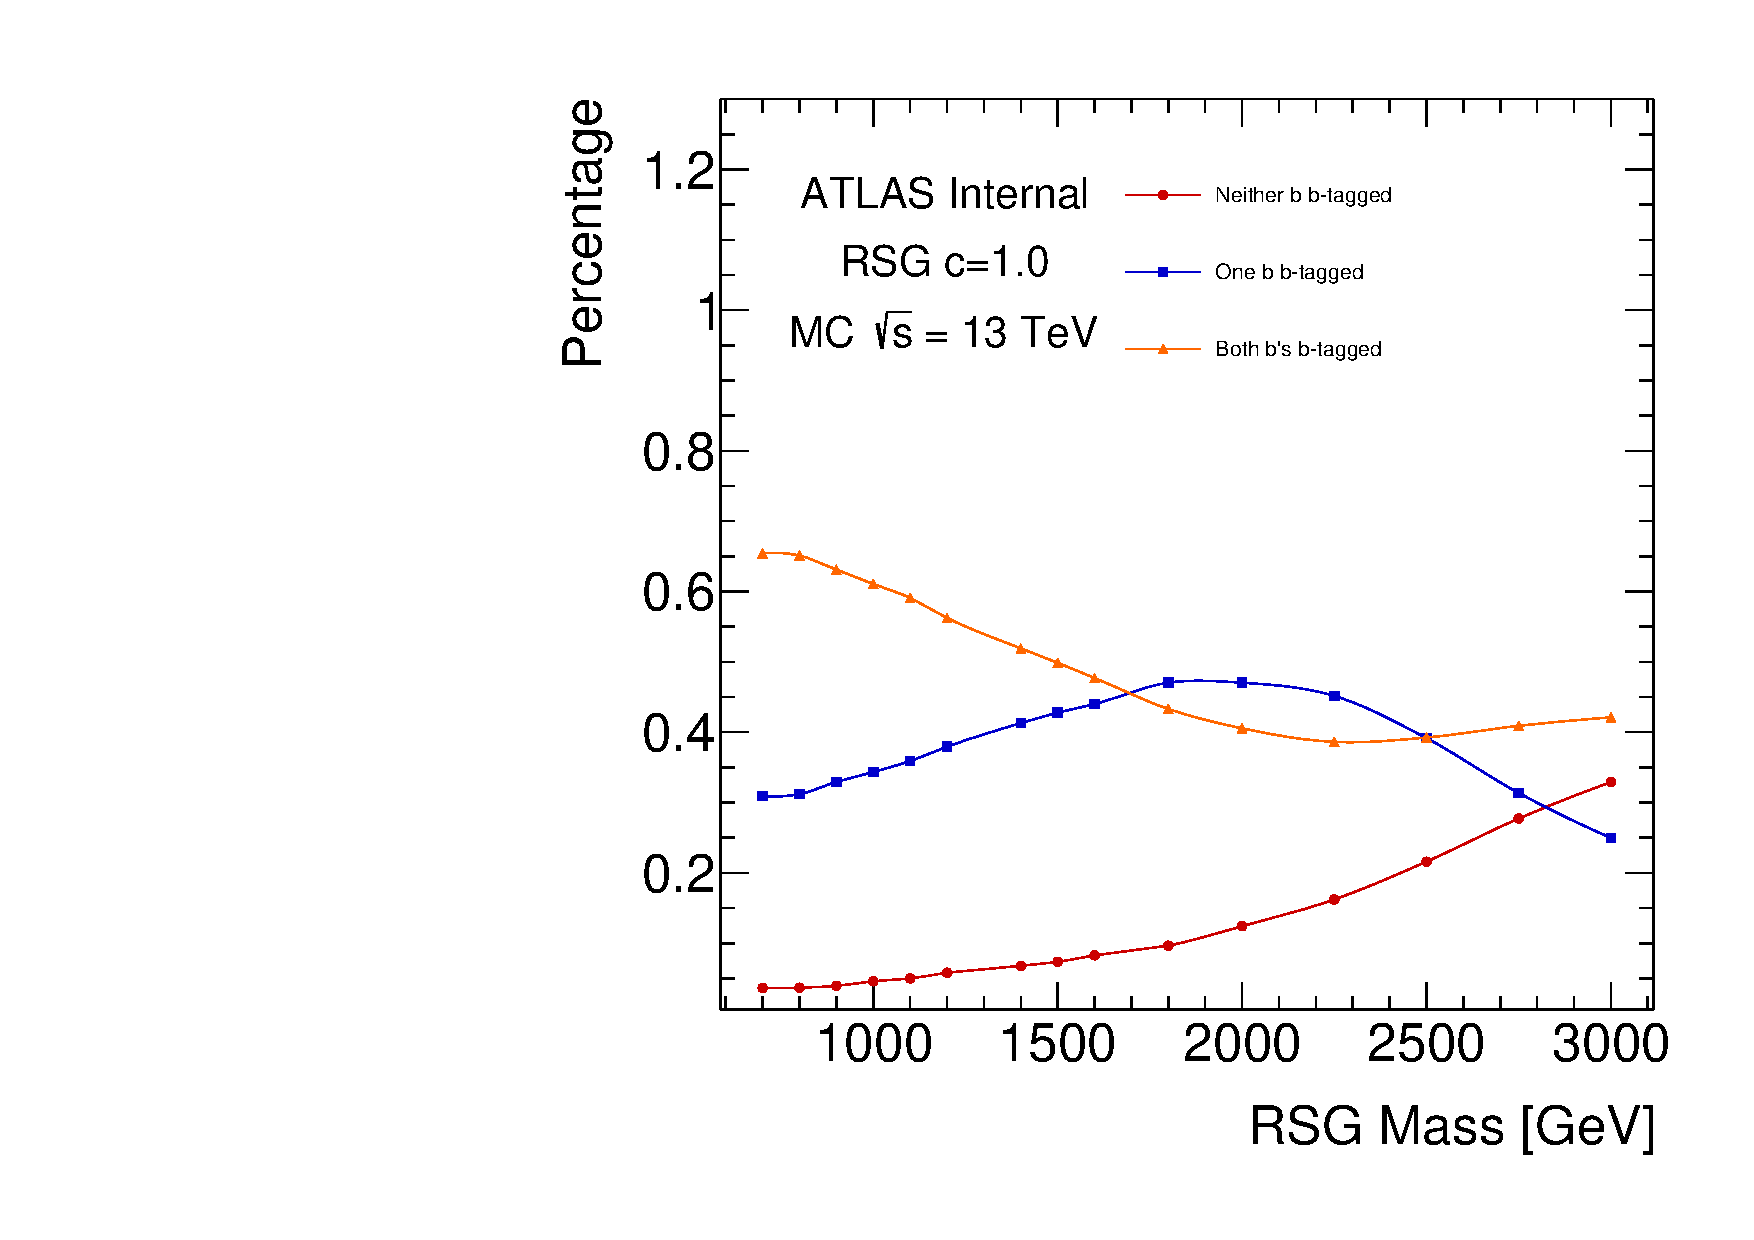
\includegraphics[angle=270, width=7cm]{figures/boosted/Appendix-Truth/truth_b-tag-matching.pdf}}}
\qquad
%\subfloat[Subleading Higgs]{{%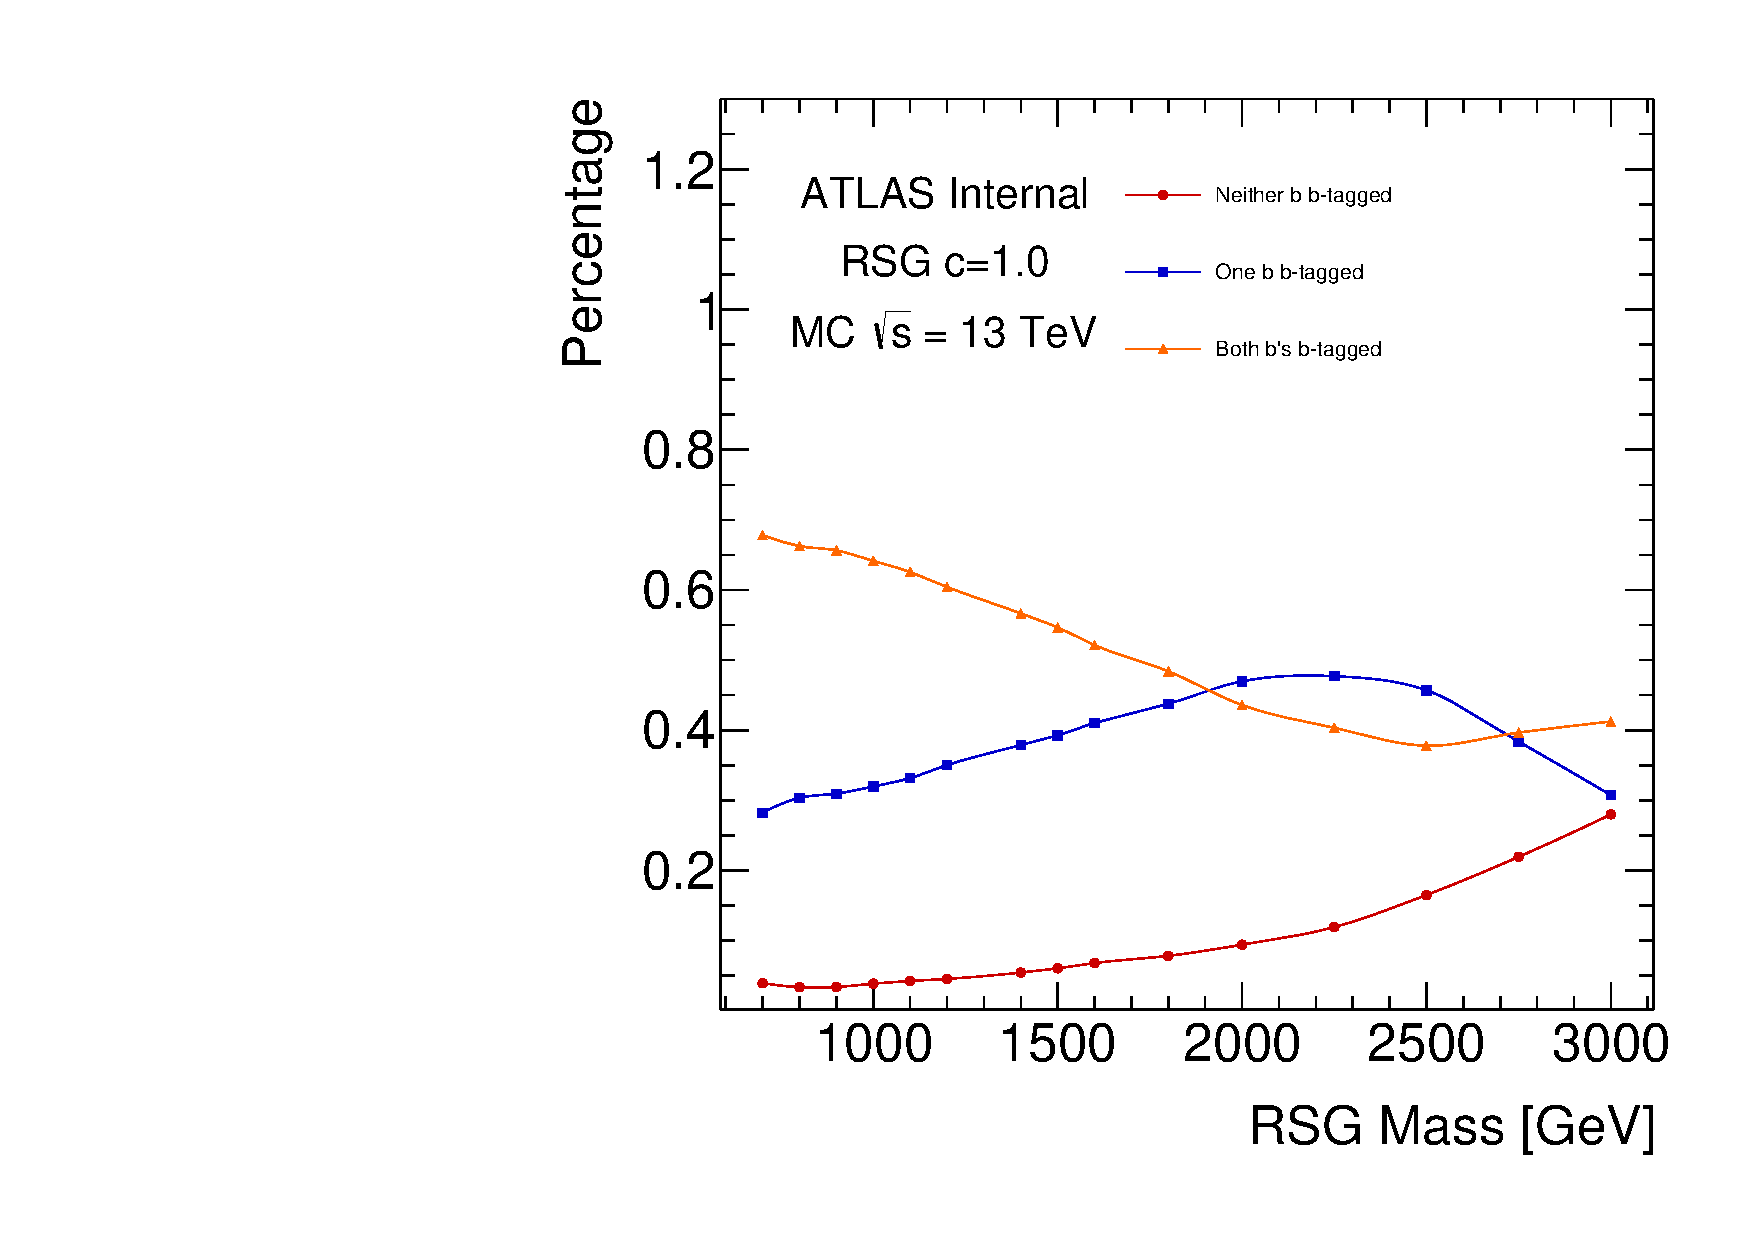
\includegraphics[angle=270, width=7cm]{figures/boosted/Appendix-Truth/truth_b-tag-matching-sublead.pdf} }}
\caption{Percentage of the time that trackjets matched to b's are b-tagged (b's inside leading Higgs on left, inside subleading on right). b-tagging is based on MV2c20 at a cut of $-0.6134$ (a working point of $77\%$). Only those cases where both b's are matched to a trackjet are considered. In the case where one b is matched to two jets, the closer of the two jets is checked against. The b's are allowed to match to the same jet.}
\label{fig:app-truth-bbtag}
\end{center}
\end{figure}
